%run:
%xelatex report.tex
%bibtex8 --wolfgang report
%xelatex report.tex

\documentclass[a4paper,12pt]{article}
\usepackage{fontspec}
\usepackage[finnish,english]{babel}
\usepackage[toc,page]{appendix}
\usepackage{pdflscape}
\usepackage{enumitem}

\usepackage[backend=bibtex,bibstyle=verbose,citestyle=authoryear-ibid]{biblatex}
\addbibresource{bibliography.bib}

\interfootnotelinepenalty=10000

\title{\vspace*{-3cm}Smoke Gets in Your Eyes\\\Large{Miniproject final report}}
\author{Niko Ilomäki \and Niclas Joswig \and Sampo Savolainen}
\date{October 29, 2018}

\begin{document}

\maketitle

\section{Introduction}

The miniproject Smoke Gets in Your Eyes concentrates on wildfires and their effects on air quality. The starting point was the dataset 1.88 Million US Wildfires which is available on Kaggle. Given the effects of wildfires on air quality, air quality data was a natural pairing for the wildfire data. There is an abundance of freely available measurement data on air quality published by the U. S. Environmental Protection Agency (EPA).

There are indications that problems with wildfires are only worsening in the United States.\footnote{See for example the recent article \url{https://fivethirtyeight.com/features/wildfires-in-the-u-s-are-getting-bigger/}.} The adverse health effects of wildfire smoke have also been noted in media recently.\footnote{See e.g. \url{https://www.washingtonpost.com/news/capital-weather-gang/wp/2018/08/07/wildfire-smoke-is-wreaking-havoc-on-the-air-quality-in-the-western-u-s}} As wildfires grow in size and quantity, new solutions that help managing their impact would certainly be helpful.

Although the data used in the project pertains to the United States, a similar approach would work with other countries given similar measurement data. In Europe, countries such as Sweden and Greece have suffered greatly from wildfires recently.

\section{Target audience}

While the solution could also be repurposed for individual use (e.g., in the form of a website), the primary target audience is government agencies which could use the model to provide earlier warnings of large changes in air quality. Because the predictions come with different confidence levels and there may be other factors to consider, it seems more reasonable to start the deployment from said agencies where the predictions would be reviewed by expert staff before wider publication.

\section{Technical details of the project}

%This section explains the technical details of implementing different aspects of the project.

\subsection{Data wrangling}

Data wrangling was accomplished using Python and the \texttt{pandas} library as well as R.

The data on wildfires are available as a SQLite database. The database contains information on a total of 1.88 million fires in the U.S. between 1992 and 2015, including the discovery and containment dates of the fire, size of the fire, location of the fire, and a host of administrative information such as the agencies and units involved in containing the fire and identifiers for the fire in different systems. We discarded most of this administrative information since it was not pertinent to the task of predicting the severity of the fire. We included the information on the location of the fire (latitude and longitude coordinates), the estimated final size of the fire (in acres and as a categorical class), and the dates of the fire (from discovery to containment). This information was read into a \texttt{pandas} data frame using a SQL query.

The air quality data we used are available from the U.S. Environmental Protection Agency. We chose to use daily summaries of AQI (air quality index) divided by county, which was the most fine-grained location distinction available. The data were available as CSV files, each file containing a year of daily summaries. The summary files included location information (state and county names and codes), measurement date, AQI reading and category, the defining parameter (the most significant pollutant in the measurement), ID code for the defining site (consisting of state and county codes and a site number), and the number of sites reporting the measurement. These summaries are available from 1980 to 2018, and we downloaded the files for years corresponding to the wildfire data (1992–2015). Each CSV file was handled as its own \texttt{pandas} data frame.

The AQI summary files posed a problem: the exact location of the measurement was not included, and having merely the county information is way too coarse as a location. Fortunately, the EPA also provides a file with information the sites involved in AQI measurements, including the location, although the site ID codes needed to be parsed from separate columns containing the state, county, and site numbers. We then proceeded to add the exact coordinates for each measurement by mapping the ID code for the defining site in the AQI data with the site's coordinates.

When we had exact location data for each AQI measurement, we combined the measurements with the wildfire data. Due to time constraints, this step was done simplistically for the data used in the ML model: for each fire, we retrieved a list of AQI measurements from the time period between the discovery and containment of the fire, narrowed them down to measurements inside a 1 by 1 degree (longitude by latitude) area centered on the fire coordinates, and chose the closest measurement (if any were present). This followed from an uncertainty in establishing how far the smoke from a wildfire could impact air quality, so we chose to focus on a relatively small area around the fire.

This simplistic approach does have several limitations. First, attaching only a single AQI reading to each fire gives only a very brief glimpse at the situation: having readings from the entire duration of a fire allows more insight into the data, and we did accomplish this for some later data analysis. Second, the way the area around the fire was defined was not ideal: the area is rectangular instead of circular, which would make more sense, and since the distance covered by 1 degree of longitude depends on the latitude, the size of the search area varied between fires. However, this rough approximation was sufficient for the purposes of this project and could be improved upon in future work.

\subsection{Data analysis and visualization}

For further analysis of the relationship of the wildfires and air quality, it was deemed necessary to use longer time series of measurements. Thus, new tools were developed, this time in R. Because mapping wildfires to measurement stations takes a long time, the data from the previous phase was taken as the starting point. To first determine whether there was a tangible relationship between the wildfires and air quality in our model, the following scheme was devised: (N.b. Plots can be found in Appendix A.)

\begin{enumerate}[itemsep=-0.5ex]
	\item Attach to each wildfire all AQI measurements from the day before the fire started to the day after the fire ended (this guarantees at least one measurement for each fire).
	\item Calculate several statistics from the series of measurements: first measurement, last measurement, average measurement, lowest measurement, and highest measurement.
	\item The difference between last and first measurement (\emph{change} in plots) should not be very indicative of the fire since they should be before and after the fire.
	\item However the difference between highest and first measurement (\emph{max\_change} in plots and below) should indicate how much worse the air quality got during (and possibly because of) the fire.
	\item On the other hand, difference between lowest and first measurement (\emph{min\_change} in plots) should indicate how much better the air quality got during the fire. It is assumed that the fire should not improve air quality.
	\item If the previous two differences are of similar size, it apperas very likely that the wildfires are not a good indicator for air quality in our model.
\end{enumerate}

Unfortunately, the results were disappointing; the two differences were indeed of similar size. Moreover, both grew with fire size, but this appears to be because larger fires last longer: they have longer time series and more variance is realized. With the two classes of largest fires (classes 5 and 6) there appeared to be some difference in favor of \emph{max\_change}, but not enough to build regression on. Thus, focus was shifted from air quality index to two gases that should be especially prevalent during wildfires: carbon monoxide and sulfur dioxide. However, results with the two gases did not impress either. First of all, they were not measured in all locations so there was not a nearby measurement for all fires; thus a subset was used. Results with carbon monoxide were very similar to AQI, with only class 6 fires showing inclination towards \emph{max\_change}. Sulfur dioxide measurements behaved best and would form the best starting point for future improvements. Those results do have their own issues, however, with class 5 implying (not necessarily causing) larger changes than class 6, so that part does seem suspect.

\subsection{Prediction model for wildfire severity}

The task to predict the severity of a wildfire is displayed technically as a classification problem. In the current model, we use the final size of the fire as the indicator for severity, and the model predicts the membership to seven available classes on the basis of ten input features. The classes describe intervals of area sizes, in which the wildfires with the fitting size are.

We tried to solve this problem with a variety of machine learning algorithms, such as XGBoost, Decision Trees and Linear Regression, but the best performance was achieved by Neural Networks. The structure of the network can be seen in Appendix B.

The network consists of five blocks which contain 4 layers each. Every block starts with a Dense layer that has between 256 and 1200 neurons. After the Dense layers follow Activation layers with ReLu-function, which is the currently best activation-function for deep neural networks.

To improve performance, Batchnormalization layers were added into every block in order to speed up learning and improve performance with data optimization. Overfitting the network is prevented by using Dropout layers, which have in our case low rates from $0.2$ and $0.3$. More Dropout is not needed, because the Dataset is very large, so the variety on data is huge.

After training the model with the SGDOptimizer with a learning-rate of $0.01$, a decay of $10^{-6}$ and a Momentum of $0.9$, we achieved 65\% accuracy as our best result.

Considering that there are seven classes, meaning that random choice has a probability of $1/7$ to be correct, the model delivers reasonable results.

\section{Future directions}

It seems reasonable to assume that weather conditions, most notably the direction and speed of wind, affect where the smoke impact of a wildfire is felt. Therefore integrating them into the model could be beneficial. Each fire could also be connected to multiple measurement sites, weighted by distance.

Another important aspect would be to split the prediction into individual components of the air quality index and then reconstruct the index instead of predicting the index directly. Some steps into that direction were already taken with carbon monoxide and sulfur dioxide analyses.

In predicting how severe a wildfire can get, it could be useful to explore more data than what was possible within the scope of this project. For example, it would seem reasonable to assume the size of the fire is affected by the dryness and amount of vegetation in the area. Therefore, using weather data to determine the dryness of the region the wildfire occurs in could help with the prediction. Including the type and amount of combustible vegetation in the area could perhaps be included through explicit data, if such data is available, or roughly estimated by examining the history of wildfires in the area: if fires have occurred recently, there would be less vegetation.

In terms of deploying our solution, future work could include a website that automatically updates air quality predictions for ongoing wildfires.

\section{Who did what?}

Topic selection, planning, design, and final report involved the whole team.

Sampo was mainly responsible for managing and wrangling most of the AQI data and for combining the AQI data with the wildfire data for the prediction model.

Niclas was responsible for managing the wildfire data, combining wildfire and AQI data, and building the prediction model for severity.

Niko looked further into the combined wildfire and AQI data as well as other measurement data, and did the analysis and visualization for that.

\begin{landscape}
\begin{appendices}
\section{Measurement data visualizations}
\subsection{Air quality index}
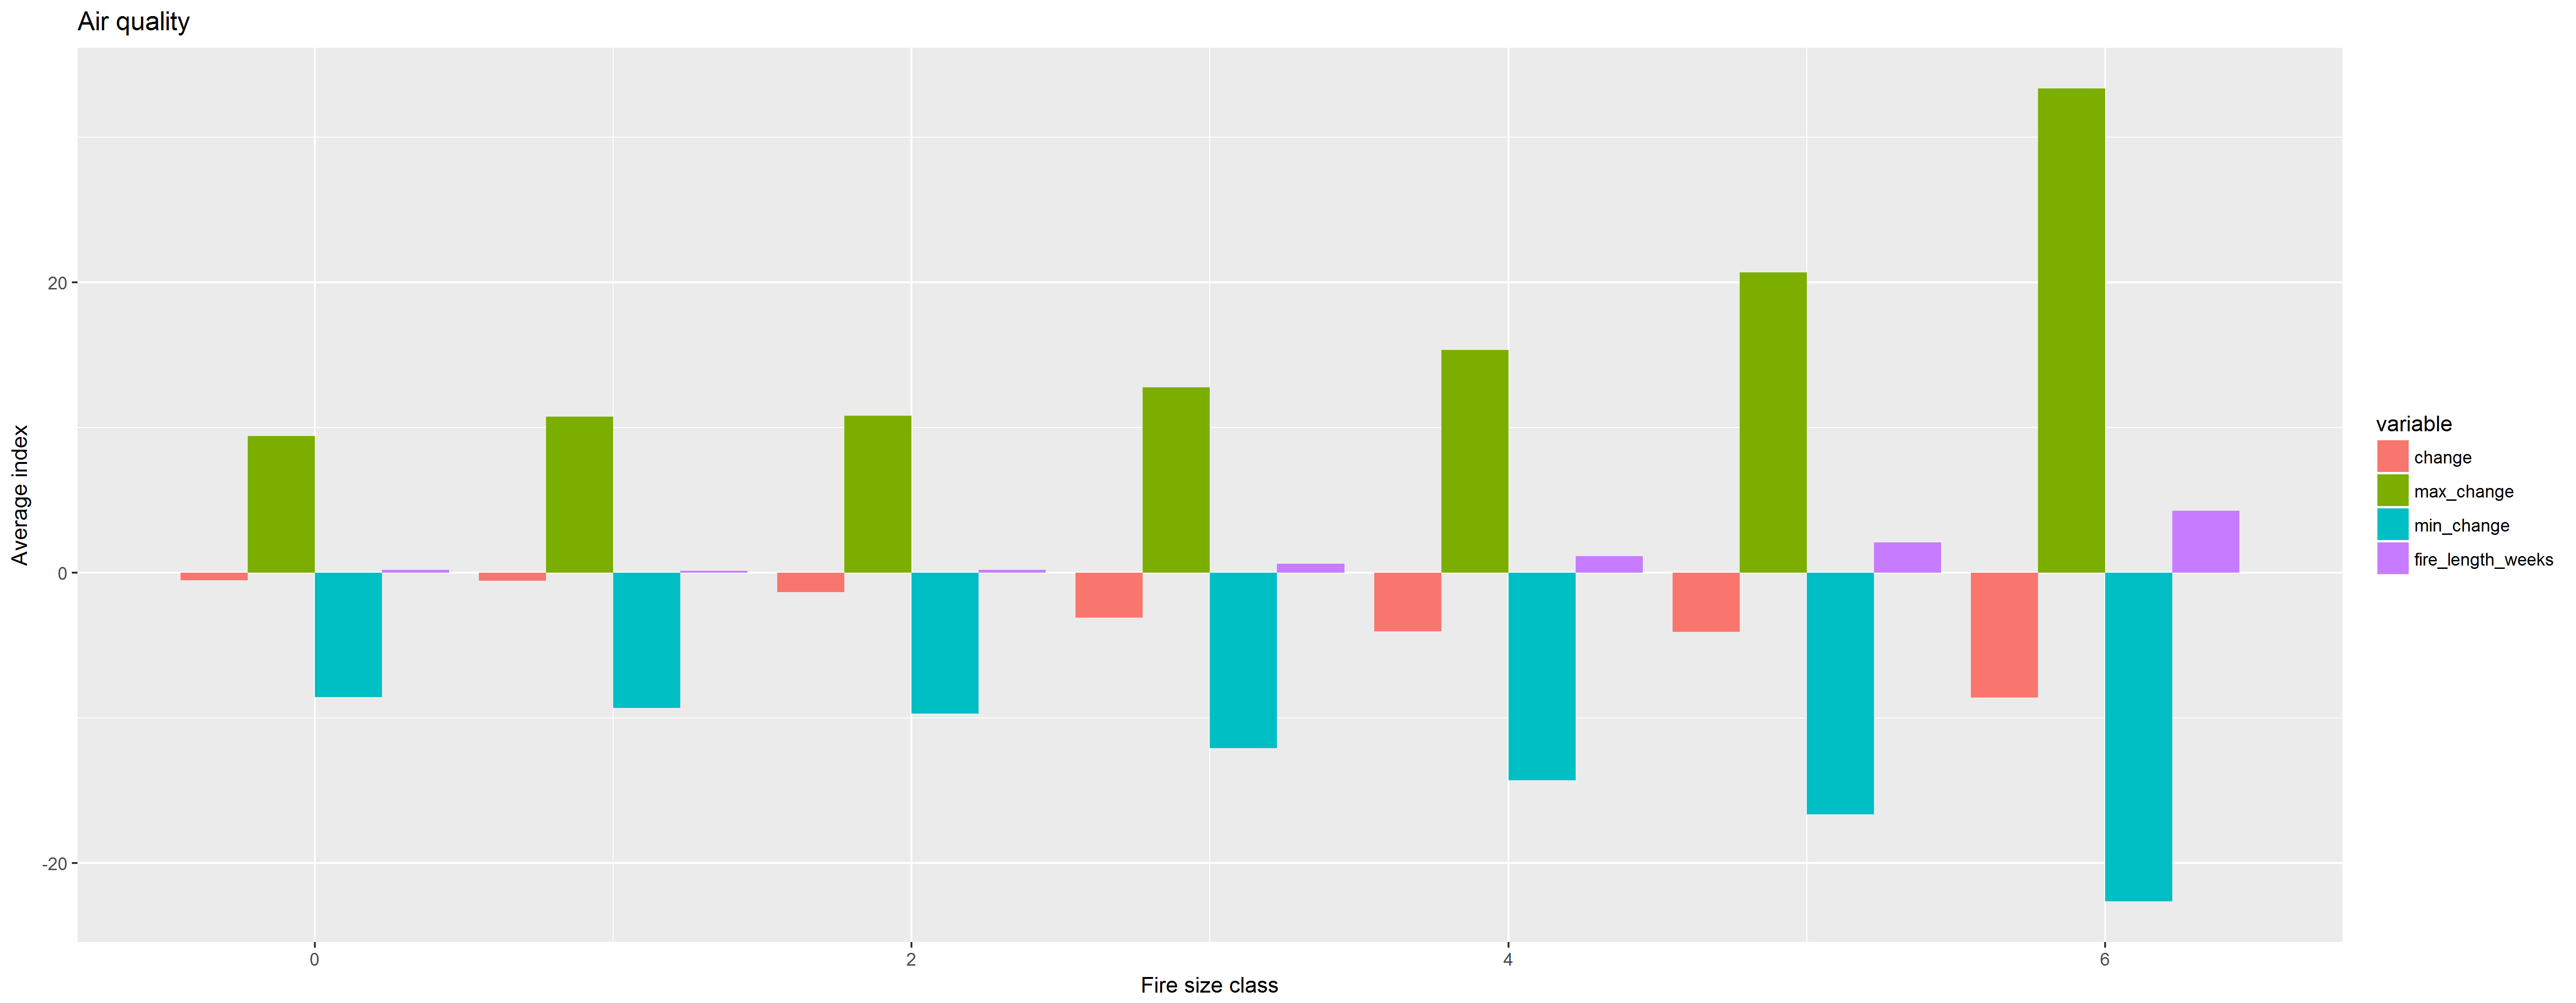
\includegraphics[scale=0.5]{aqi_time_series.png}
\subsection{Carbon monoxide}
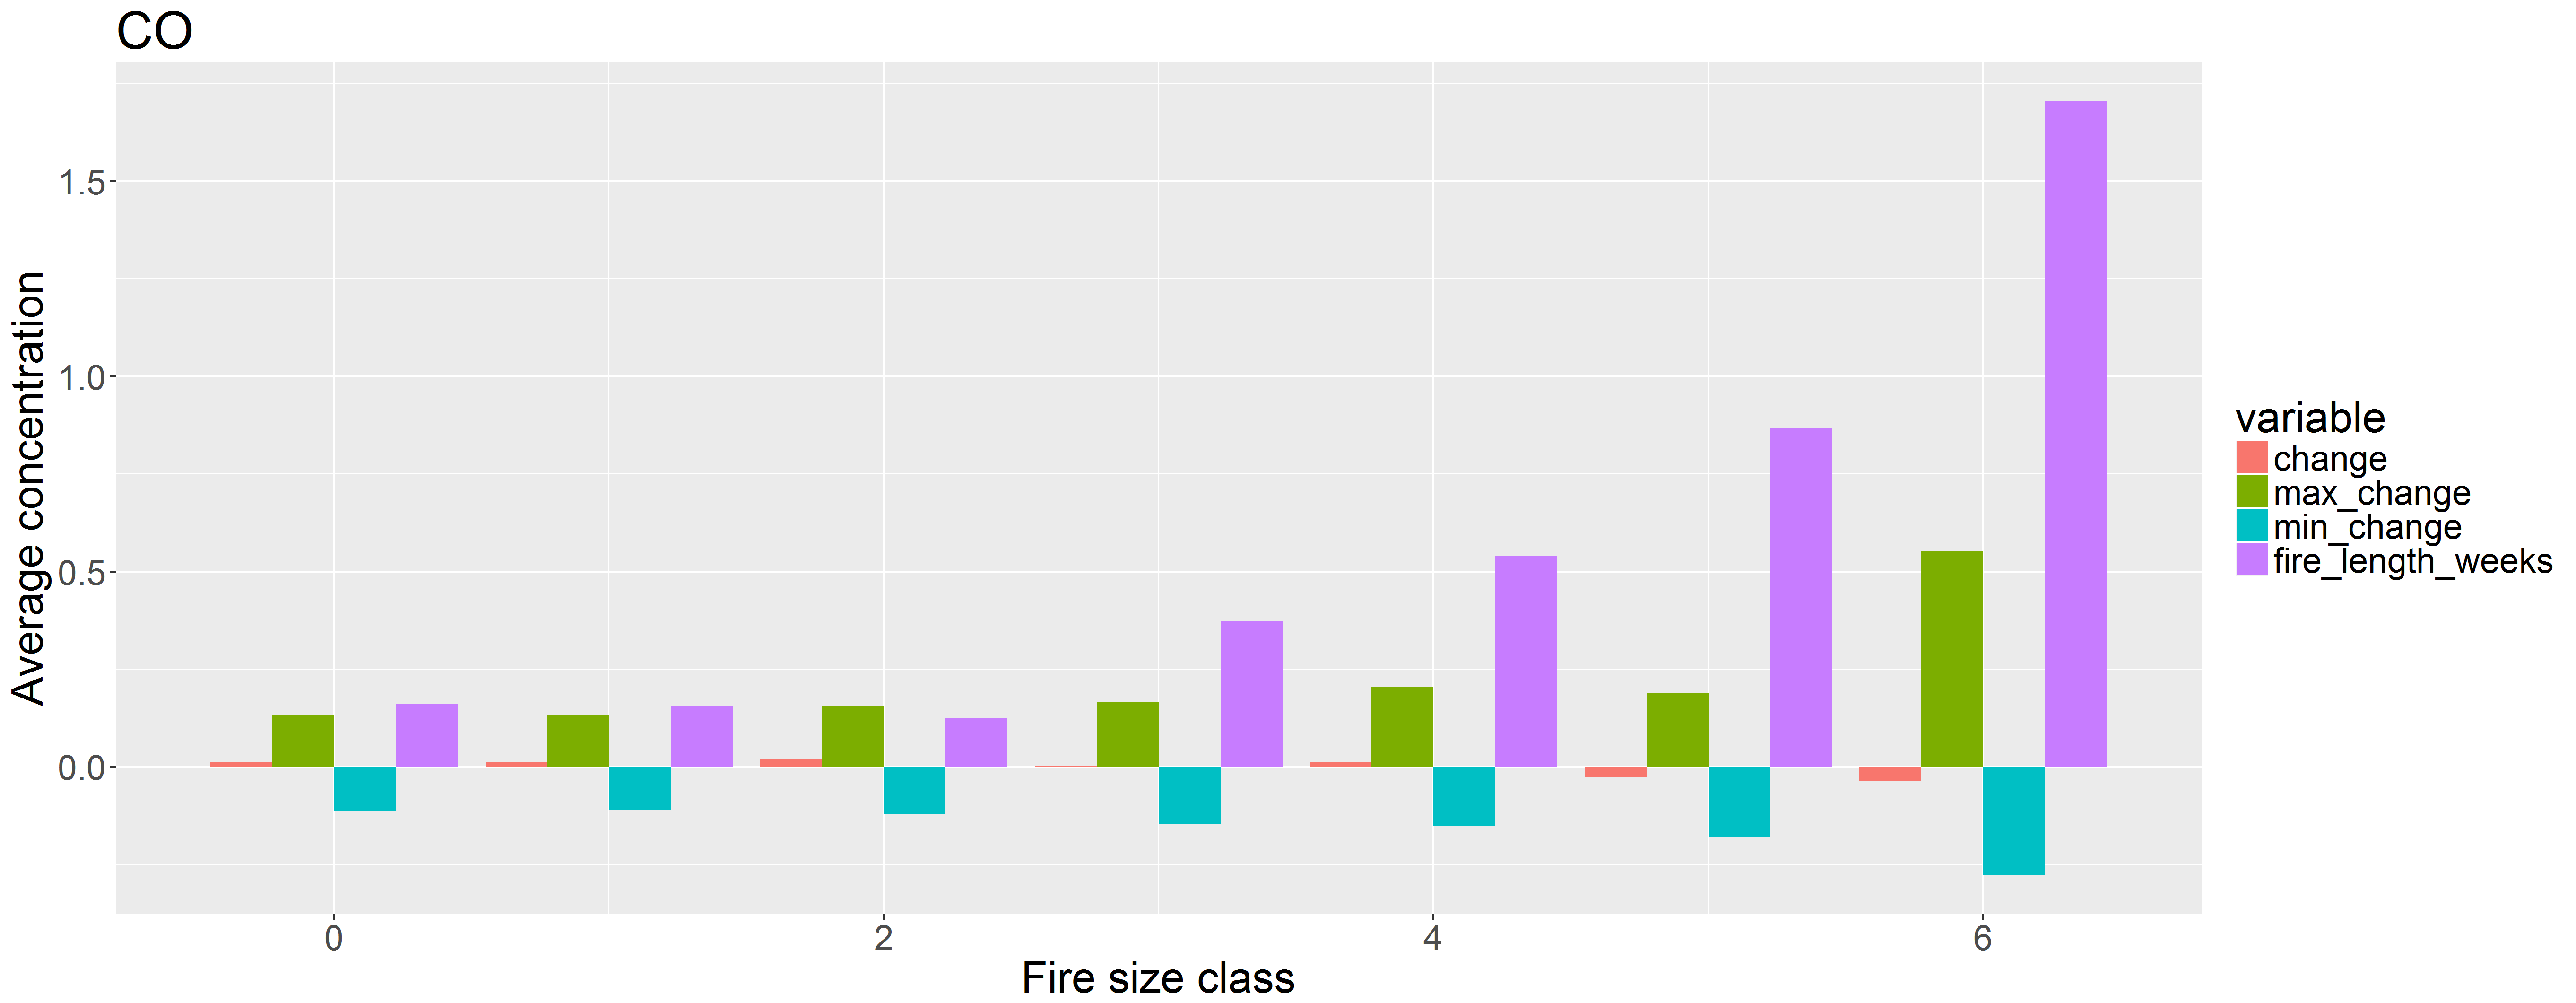
\includegraphics[scale=0.5]{co_time_series.png}
\subsection{Sulfur dioxide}
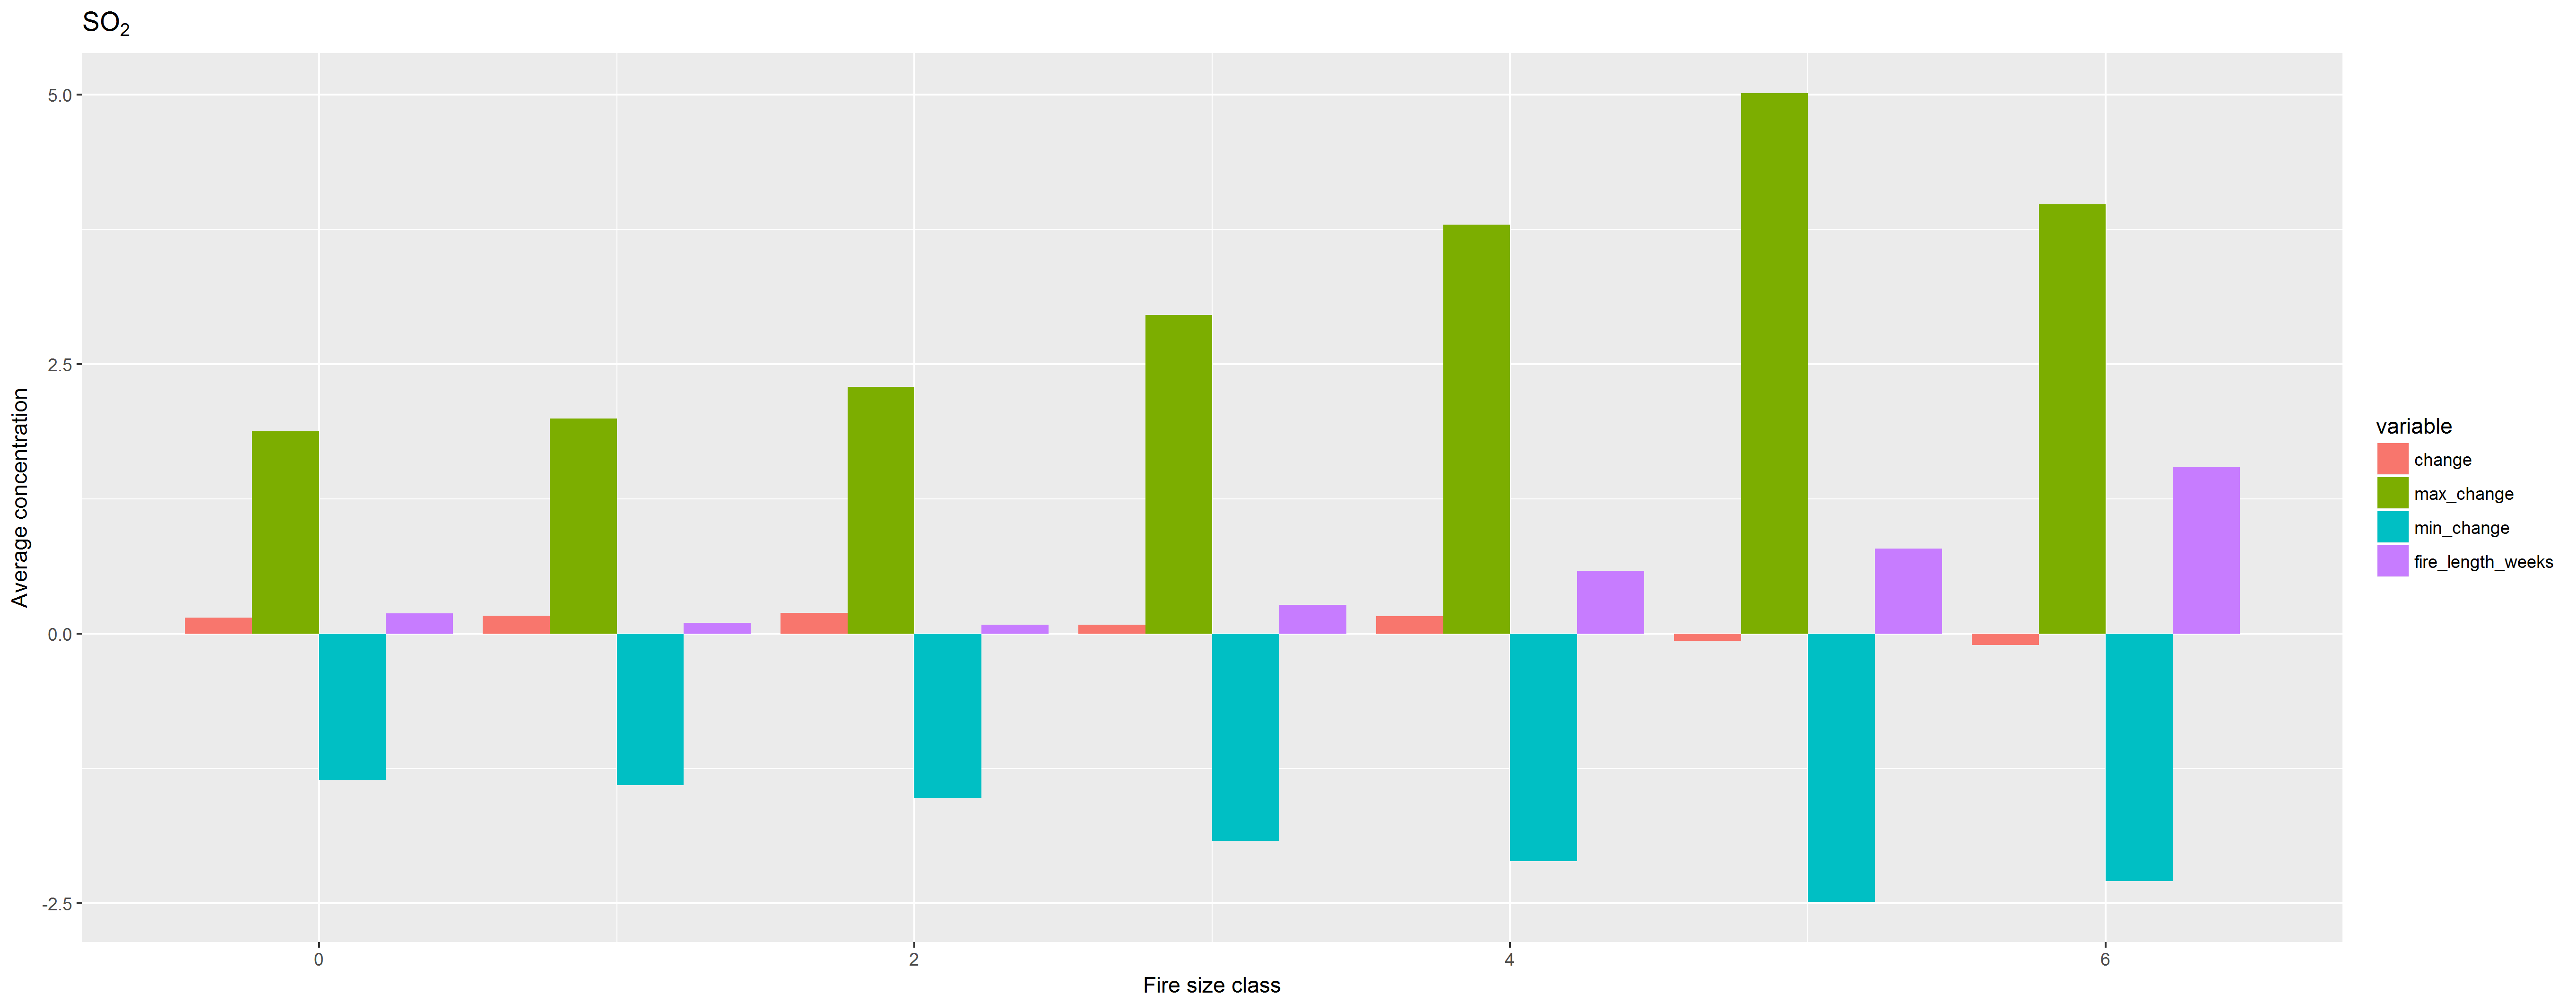
\includegraphics[scale=0.5]{so2_time_series.png}
\section{Structure of the neutral network}
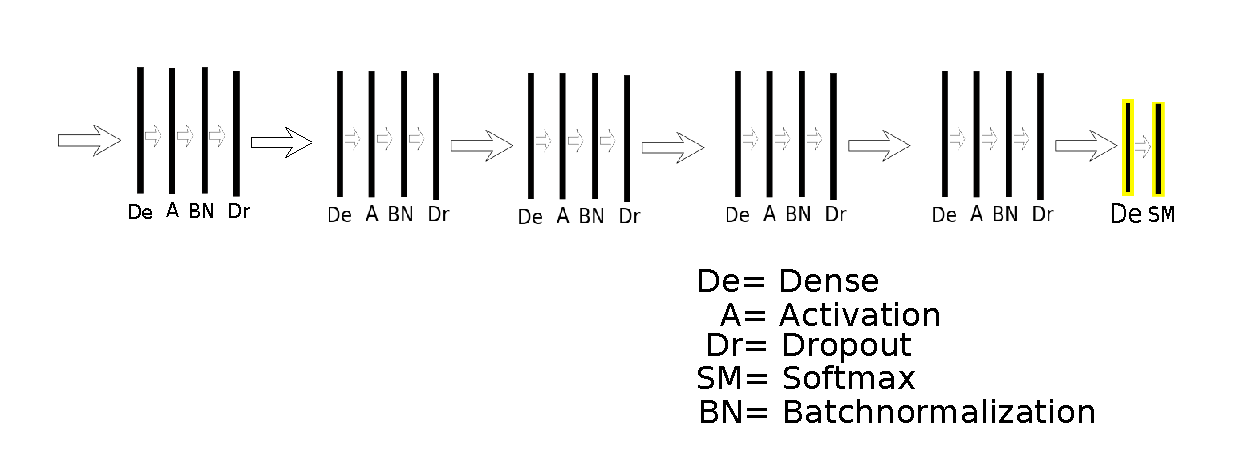
\includegraphics[scale=1]{nn.pdf}
\end{appendices}
\end{landscape}

\nocite{*}
\printbibliography[title={Bibliography},heading=bibliography]

\end{document}
